\documentclass[journal, a4paper]{IEEEtran}

\usepackage{graphicx}
\usepackage{url}
\usepackage{bm}
\usepackage{amsmath}
\usepackage{amssymb}
\usepackage[justification=centering]{caption}

% Your document starts here!
\begin{document}
\begin{titlepage}

\newcommand{\HRule}{\rule{\linewidth}{0.5mm}} % Defines a new command for the horizontal lines, change thickness here

\center 
~\\[1cm]

\includegraphics{SCUT.png}\\[2cm] 
\HRule \\[1cm]
{ \huge \bfseries The Experiment Report of \textit{Deep Learning} }\\[0.6cm] % Title of your document
\HRule \\[2cm]

\textsc{\LARGE \textbf{School:} School of Software Engineering}\\[1cm]
\textsc{\LARGE \textbf{Subject:} Software Engineering}\\[2cm]

\begin{minipage}{0.4\textwidth}
\begin{flushleft} \large
\emph{Author:}\\
Qichen Huang % Your name
\end{flushleft}
\end{minipage}
~
\begin{minipage}{0.4\textwidth}
\begin{flushright} \large
\emph{Supervisor:} \\
Mingkui Tan% Supervisor's Name
\end{flushright}
\end{minipage}\\[2cm]
~
\begin{minipage}{0.4\textwidth}
\begin{flushleft} \large
\emph{Student ID:}\\
201920142806
\end{flushleft}
\end{minipage}
~
\begin{minipage}{0.4\textwidth}
\begin{flushright} \large
\emph{Grade:} \\
Graduate
\end{flushright}
\end{minipage}\\[2cm]

% If you don't want a supervisor, uncomment the two lines below and remove the section above
%\Large \emph{Author:}\\
%John \textsc{Smith}\\[3cm] % Your name

%----------------------------------------------------------------------------------------
%	DATE SECTION
%----------------------------------------------------------------------------------------

{\large \today}\\[2cm] % Date, change the \today to a set date if you want to be precise


%----------------------------------------------------------------------------------------

\vfill % Fill the rest of the page with whitespace

\end{titlepage}

% Define document title and author
	\title{Recommender System Based on Matrix Decomposition}
	\maketitle

% Write abstract here
\begin{abstract}
Recommender System aims to recommend items to users by predicting rating scores for items by users. 
We utilize Matrix Decomposition, an algorithm of Collaborative Filtering, to deal with Recommender System problem.
For training Matrix Decomposition model, Alternative Least Square, an optimization method, is introduced to learn parameters of model.
We conduct experiment on MovieLens-100k dataset and reach satisfying performance in a few iterations.
\end{abstract}

% Each section begins with a \section{title} command
\section{Introduction}
	% \PARstart{}{} creates a tall first letter for this first paragraph
\IEEEPARstart{R}{ecommender} System is a popular machine learning problem which is used to recommend items to users.
In most cases, Recommender System is regard as a task predicting a score matrix $R_{n\_users,n\_items}$ where each row represents the scores rated by a specific user, and each column represents the scores of a specific items rated by different users.
A higher score means that the item corresponding to its column gains more affection from the user corresponding to its row.
Thus, given a score matrix $R_{n\_users,n\_items}$, we can recommend some high-score items to a specific user based on the row in matrix that represents it.

Collaborative Filtering is a group of Recommender System algorithm whose idea is to predict score matrix based on existing scores rated by users.
In this experiment, we implement Recommender System with Matrix Decomposition which is a common algorithm in Collaborative Filtering.
It assumes that the rating scores can be computed with some underlying features of users and items.
So our objective is to learn the underlying features of users $P_{n\_user,K}$ and items $Q_{n\_items,K}$, where $K$ represents the number of features.

Our motivation is to 1) explore the construction of recommended system, 2) understand the principle of matrix decomposition, 3) understand the theory of Alternative Least Square algorithm, 4) Construct a recommendation system under small-scale dataset.
% Main Part
\section{Methods and Theory}
\subsection{Matrix Decomposition}
Matrix Decomposition breaks the score matrix $R_{n\_users,n\_items}$ into two smaller matrices $P_{n\_user,K}$ and $Q_{n\_items,K}$ representing the underlying features of users and items respectively.
When it comes to prediction, the predicted value of $R_{ui}$ is calculated as $P_u$ times ${Q_i}^T$, where $P_u$ is $u$ th row of $P_{n\_user,K}$ and $Q_i$ is $i$ th row of $Q_{n\_items,K}$.
In other words, the predicted score matrix is calculated as $R_{n\_user,n\_items}=P_{n\_user,K}\times {Q_{n\_items,K}}^T$

Since the ground truth score matrix is usually incomplete and nonexistent scores are filled with zeros, these nonexistent scores should not be taken into account when calculating loss function.
Thus, we define the loss function as $\mathcal{L}=\frac{1}{2}\sum\limits_{(u,i)\in{S}}{(\hat{y}_{u,i}-y_{u,i})^2}$, where $S$ is the subscript set of existent scores.
To prevent overfitting to the training set of scores, penalty terms $\lambda \sum\limits_u{||P_u||^2}$ and $\lambda \sum\limits_i{||Q_i||^2}$ are added into loss function.
Then, the loss function now looks like $\mathcal{L}=\frac{1}{2}\sum\limits_{(u,i)\in{S}}{(\hat{y}_{u,i}-y_{u,i})^2}+\lambda \sum\limits_u{||P_u||^2}+\lambda \sum\limits_i{||Q_i||^2}$.
\subsection{Alternative Least Square}
Given the loss function above, we can optimize it using gradient descent.
However it turns out to be slow and costs lots of iterations.
Note that if we fix matrix $P$ and treat them as constants, then the objective is convex function of $Q$ and vice versa.
Therefore we alternatively optimize $P$ and $Q$ by fixing the other as constant and setting partial derivative to zero.
This approach is known as Alternating Least Square(ALS).
The details of ALS algorithm are shown in Table \ref{tab:ALS}:
\begin{table}[!hbt]
  \centering
  \caption{Alternative Least Square}
  \label{tab:ALS}
  \tabcolsep = 1pt
  \resizebox{\columnwidth}{!}{
  \begin{tabular}{llp{0.4\columnwidth}}
    \hline
    \textbf{Input:} \\
     & incomplete score matrix $R$ \\
     & number of features $K$ \\
     & penalty factor $\lambda$ \\
     & number of iteration $n_{iter}$\\
    \textbf{Steps:} &  \\
    1: & initialize matrices $P$ and $Q$ \\
    2: & \textbf{for} $n=1\dots n_{iter}$\\
    3: & \quad{}\textbf{for} $u=1\dots n\_users$ \textbf{do} \\
    4: & \qquad{}$P_u=({Q_*}^TQ_*+\lambda I)^{-1}{Q_*}^TR_u$ //& $Q_*$ is modified from $Q$ that $i$ row is zero vector if $R_{u,i}$ is zero and $R_u$ is $u$ th row of $R$\\
    5: & \quad{}\textbf{end for} \\
    6: & \quad{}\textbf{for} $i=1\dots n\_items$ \textbf{do} \\
    7: & \qquad{}$Q_i=({P_*}^TP_*+\lambda I)^{-1}{P_*}^T{R^T}_i$ //& $P_*$ is modified from $P$ that $u$ row is zero vector if $R_{u,i}$ is zero and ${R^T}_i$ is $i$ th column of $R$\\
    8: & \quad{}\textbf{end for} \\
    9: & \textbf{end for} \\
    \textbf{Output:} \\
    & predicted score matrix $\hat{R} = P \times Q$ \\
    \hline
  \end{tabular}}
\end{table}
\section{Experiments}
\subsection{Dataset}
The rating scores data come from MovieLens-100k, with 10000 scores rating from 943 users to 1682 movies. 
In this dataset, each user rates 20 scores at least and we utilize "ua.base" and "ua.test" as our training set data and validation set data separately.
It splits the whole data with exactly 10 ratings per user in the validation set.
\subsection{Implementation}
The experiment steps of ALS algorithm are as follows:
\begin{enumerate}
  \item Read the training data set and validation data set. Populate the original scoring matrix $R_{n\_users,n\_items}$ against the raw data, and fill 0 for null values.
  \item Initialize the user factor matrix $P_{n\_user,K}$ and the item (movie) factor matrix $Q_{n\_items,K}$, where $K$ is the number of potential features.
  \item Determine the loss function and the penalty factor $\lambda$.
  \item Use ALS optimization method to decompose the sparse user score matrix, get the user factor matrix and item (movie) factor matrix:
      \begin{enumerate}
        \item With fixed item factor matrix, find the loss partial derivative of each row (column) of the user factor matrices, set the partial derivative to be zero and update the user factor matrices.
        \item With fixed user factor matrix, find the loss partial derivative of each row (column) of the item factor matrices, set the partial derivative to be zero and update the item
        \item Calculate the $\mathcal{L}_{validation}$ on the validation set, comparing with the $\mathcal{L}_{validation}$ of the previous iteration to determine if it has converged.
      \end{enumerate}
  \item Repeat step 4. several times, get a satisfactory user factor matrix $P$ and an item factor matrix $Q$, Draw a $\mathcal{L}_{validation}$ curve with varying iterations.
  \item The final score prediction matrix $\hat{R}_{n\_users,n\_items}$ is obtained by multiplying the user factor matrix $P_{n\_user,K}$ and the transpose of the item factor matrix $Q_{n\_items,K}$.
\end{enumerate}

In this experiment, both users factor matrix $P_{n\_user,K}$ and items factor matrix $Q_{n\_items,K}$ are initialized randomly. 
The number of feature $K$ and $\lambda$ are set as 40 and 0.5 respectively.

The curve of loss function of training set and validation set during training iteration is pictured in Fig.\ref{fig:loss}.
\begin{figure}[!hbt]
		\begin{center}
		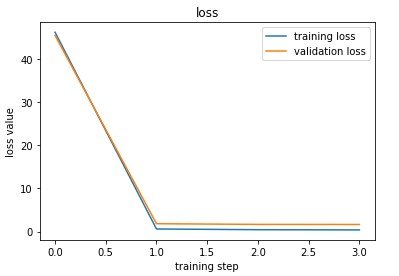
\includegraphics[width=\columnwidth]{Recommend_System_loss}
		\caption{Training set loss and validation set loss during training iteration}
		\label{fig:loss}
		\end{center}
	\end{figure}
\section{Conclusion}
In this paper, we introduce Recommend System and a kind of Collaborative Filtering algorithm, Matrix Decomposition, to implement it.
As the name means, the target Matrix is broken into two smaller features matrices to train and predict.
Also, we introduce Alternative Least Square algorithm and utilize it to learn our model.
Comparing to gradient descent, ALS algorithm can quickly get to the same performance without numbers of iterations.
\end{document}
